%% This is an example first chapter.  You should put chapter/appendix that you
%% write into a separate file, and add a line \include{yourfilename} to
%% main.tex, where `yourfilename.tex' is the name of the chapter/appendix file.
%% You can process specific files by typing their names in at the 
%% \files=
%% prompt when you run the file main.tex through LaTeX.

\chapter{Proposal and Methodology}

\section{Terminology}
In the current work and by other authors also training and learning is used interchangeably. Let me loosely define some frequently used terms and concepts in the Machine Learning arena.

\section{Data Augmentation}
Data augmentation  is a key in image based deep leaning application. This make the model robust to different object sizes, logically possible  additional training image generation via application of various image modification such as flipping horizontally \footnote{Many time flipping image vertically does not make sense in real world scenarios, wherever it makes sense, it can be done as well.}, shear, distortion, change in color intensity. In \cite{liu2016ssd} authors mentioned application of flipping each image randomly horizontally with probability of 0.5, this ensures objects appear on left and right with similar likelihood.

\section{Non-Maximum Suppression (NMS)}
During inference time, SSD predicts, a large number of boxes in a cluttered manner. To prune most of them, a technique called \textit{non-maximum suppression} is applied. This technique discards those boxes having lebel confidence less than a threshold and IoU less than a defined threshold. \footnote{Usually 0.45 is used as IoU threshold}. After discarding such boxes, only top \textit{N} predictions are returned which ensures most likely predictions.
\\*\textbf{Epoch:}
During the learning the network sees the set of samples several times. During the training, presenting the network entire set of sample once is known as an epoch. So an epoch represents one iteration over entire dataset.
\\*\textbf{Batch and batch size:}
Mainly because of two reasons we can not pass the entire dataset to the network for the training purpose at once. Firstly, datasets by nature most of the time are huge. Let it be image data or some other textual data, in many scenarios it is not possible to feed all the data because of hardware constraints, such as not enough RAM to hold entire dataset.
Secondly to update weight during training process, network has to wait for a very very long time to calculate the delta weight after processing all the input data. To solve this problem usually the full dataset is split into several small batches and number of samples within each small batch is known as 
Batch and batch size.
\\*\textbf{Iterations:} 
Number of batches that a neural network process to complete a single epoch.
The number of  iterations, batch size and  number of data samples in the dataset is given by, the below expression.
\begin{equation}
    D = B * I
\end{equation}
Where D is the total number of samples in the dataset.
\\*B is the number of samples in the mini batch that is fed to the network at once.
\\*I is the  total number of batches the network process in a single epoch.

Larger batch size requires more computational resource and achieves faster completion, in contrast smaller batch size leads to more generalization. In this regards, Yann  LeCun humorously said
\begin{quote}
``Training with large mini batches is bad for your health. More importantly, it's bad for your test error.  Friends, don't let friends use mini batches larger than 32.''
\end{quote}   
The empirical study of the performance of mini-batch stochastic gradient descent in \cite{masters2018revisiting} show that, the team obtained the best training stability and generalization performance using small batch sizes, for a given computational cost, across a wide range of experiments they conducted. In all cases they have achieved the best results with batch sizes m = 32 or smaller.
\\*\textbf{Intersection Over Union:}
Intersection Over Union (IOU) is a measure similar to Jaccard Index that measures the overlap ratio between two bounding boxes. It evaluates the ratio between area of  overlapping area between two BBs and area of union between them.

\begin{equation}
    IoU = \frac{area\: of\: overlap} {area\: of\: union} =
\end{equation}

\begin{center}
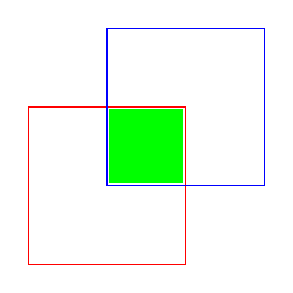
\begin{tikzpicture}
\draw [red] (0, 0) rectangle (2, 2);
\draw [blue] (1.0, 1.0) rectangle (3.0, 3.0);
\begin{scope}
	\fill[green] (1.03, 1.03) rectangle (1.97, 1.97);
\end{scope}
\end{tikzpicture}

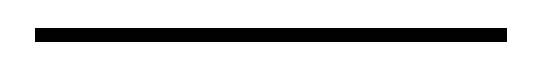
\begin{tikzpicture}
    \draw[line width=5pt,fill=black] (0,2) -- (6,2);
\end{tikzpicture}\vspace{0.2cm}%

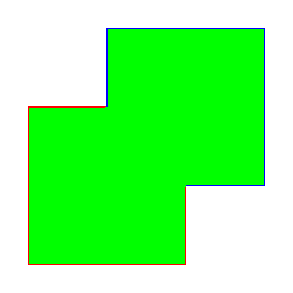
\begin{tikzpicture}
    \filldraw [draw=red,fill=green] (0, 0) rectangle (2, 2);
    \filldraw [draw=blue,fill=green] (1.0, 1.0) rectangle (3.0, 3.0);
    %\begin{scope}
			\fill[green] (0.98, 0.98) rectangle (2.0, 2.0);
		%\end{scope}
\end{tikzpicture}
\end{center}

% This is an example of how you would use tgrind to include an example
% of source code; it is commented out in this template since the code
% example file does not exist.  To use it, you need to remove the '%' on the
% beginning of the line, and insert your own information in the call.
%
%\tagrind[htbp]{code/pmn.s.tex}{Post Multiply Normalization}{opt:pmn}
